\chapter{Results}

The aim of the methods described in this thesis are to provide tools to query the disequilibrium of sequence evolution. 

In this chapter, the results from four experiments are presented. 

\section{Synthetic Data}

\subsection{Test for Disequilibrium}

 

To determine whether a given LRT statistic is significant requires establishing the appropriate null distribution. Statistical theory states that under certain conditions, the LRT statistic will be $\chi^2_{df}$ distributed with degrees freedom (df) equal to the difference in the number of free parameter between the models. In which case, one can obtain the p-values for a given LRT statistic simply from the analytical distribution. However, the behaviour of my test with real finite data is unknown. When considering the use of mixed discrete- and continuous-time Markov process is a deviation from convention, it is especially important to establish whether the test statistic is consistent with theoretical expectations. 

The distribution is closer to theoretical expectations for longer sequences, depicted in Figure \ref{fig:synthetic/lrt/197113-long_seq}. For alignments of length 300bp, shown in Figure \ref{fig:synthetic/lrt/197113-long_seq}a, the distribution of LRT statistic yields an excess of small p-values. Consequently, the data points of the Quantile-Quantile plot fall well below the diagonal line. Owing to increasing the power of the test, the distribution of p-values for longer alignments, illustrated in Figure \ref{fig:synthetic/lrt/197113-long_seq}b, is less skewed. Overall, the data points fall much closer to the diagonal line. It is worth noting that consistency with the theoretical distribution is most important for the smaller p-values. In Figure \ref{fig:synthetic/lrt/197113-long_seq}b, for quantiles corresponding to a significant test statistic (i.e. the bottom left corner where $p<0.05$), the distribution is very close to the theoretical distribution. This means that the chance of a false-positive is more or less in line with statistical expectations (5\%). Now, consider the distribution of p-values for $p>0.05$. Even though the distribution is not uniform, using the $\chi^{2}$ distribution, a non-significant result would still yield a non-significant p-value (true-negative). Thus, for some longer alignments, it may be suitable to assume the LRT statistics are $\chi^{2}$ distributed and in turn, obtain the p-value simply from analytical distribution. 



\begin{figure}[htbp]
\centering
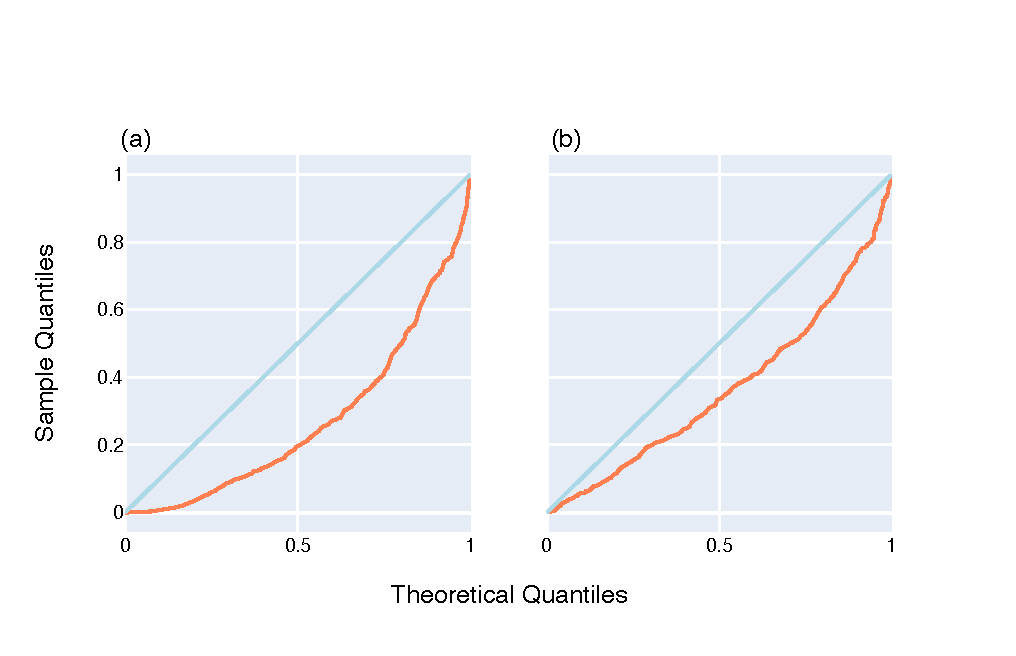
\includegraphics[width=\textwidth]{figures/plots/synthetic/lrt/197113_332182_17210-long_seq.pdf}
\caption[Increasing the length of the alignments gives a distribution of $\hat p-$ values closer, but not consistent with theoretical expectations]{\textbf{Increasing the length of the alignments gives a distribution of $\hat p-$ values closer, but not consistent with theoretical expectations.} The Quantile-Quantile (Q-Q) plots compare the $\hat p$-value distribution of the test for existence in stationary simulated data to the uniform distribution (pink line). Theoretical expectation is illustrated by the diagonal (blue line). Q-Q plot for \textbf{(a)} synthetic alignments of length $300$bp, \textbf{(b)}, synthetic alignments of length $30,000$bp. Each data set contains 1,000 synthetic stationary alignments. Both data sets shown are generated from the same high JSD, high entropy seed. The other seeds exhibited the same pattern, the result is shown in the appendix Figure \ref{fig:synthetic/lrt/all-seeds}.}
\label{fig:synthetic/lrt/197113-long_seq}
\end{figure}

Figure \ref{fig:synthetic/lrt/197113-long_branch} shows that increasing the branch length of sequences did not alter the distribution of LRT statistic. The distribution of LRT with and without branch scaling is depicted in Figures \ref{fig:synthetic/lrt/197113-long_branch}a and \ref{fig:synthetic/lrt/197113-long_branch}b respectively. The distributions are almost identical, which is further illustrated with a Quantile-Quantile plot comparing the distributions directly to each other, included in the \hyperref[Appendices]{Appendices} (see fig. ). It is important to note that this result is conditioned on constraints imposed on how much branch lengths could be changed. It is possible that allowing branch lengths to exceed $d=0.6$ and in turn, further increasing the number of events, would alter the distribution of the statistic.


\begin{figure}[!ht]
\centering
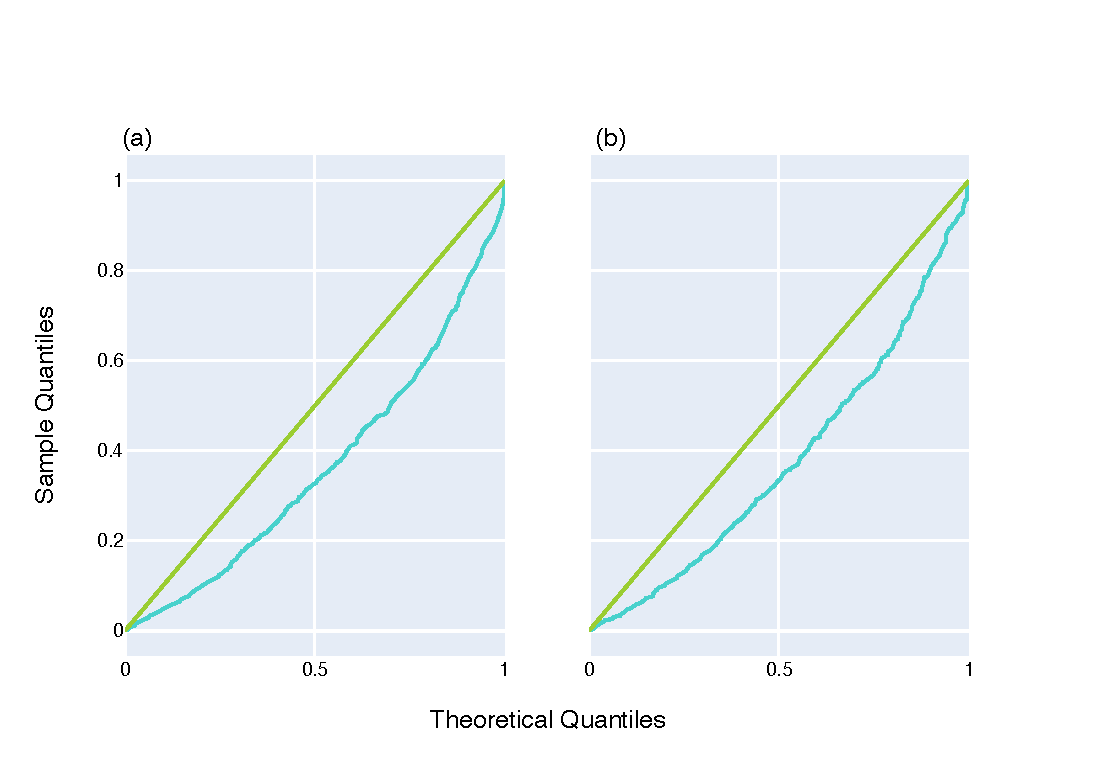
\includegraphics[width=\textwidth]{figures/plots/synthetic/lrt/197113_332182_17210-long_branch.pdf}
\caption{\textbf{Increasing the branch length to by a factor of 3 does not change the distribution of LRT p-values.} Quantile-Quantile plot comparing the distribution of the LRT p-values to the uniform distribution. \textbf{a}, simulated alignments of length 3000, \textbf{b}, simulated alignments of length 3000 with branch lengths scaled by a factor of 3. The data set was generated from the high JSD, high entropy seed.}
\label{fig:synthetic/lrt/197113-long_branch}
\end{figure}

\subsection{Published Tests}
Squartini and Arndt 


\begin{figure}
\centering
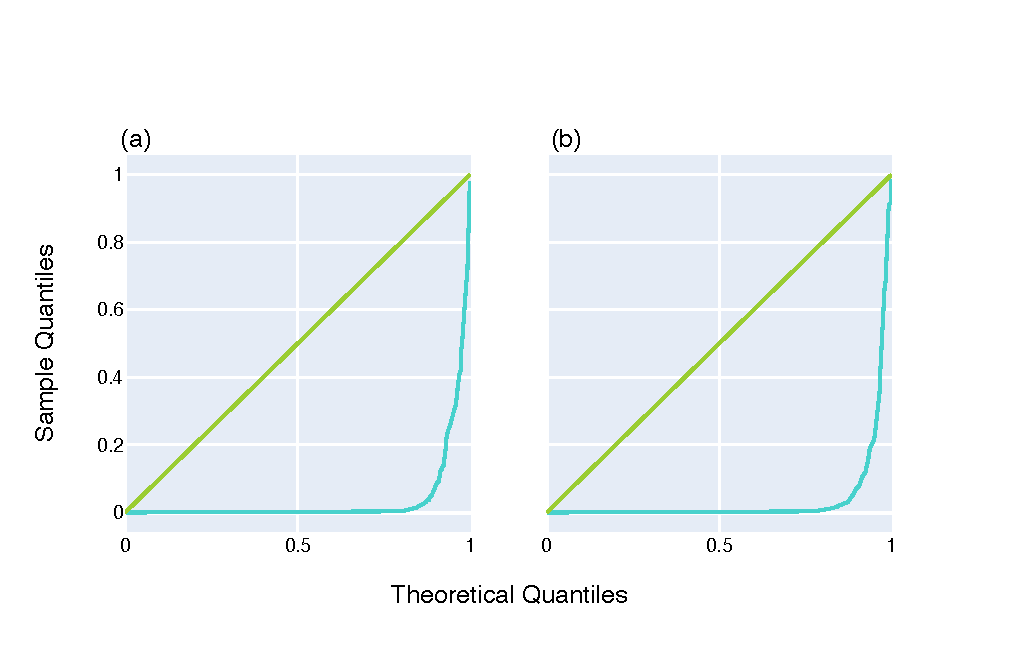
\includegraphics[width=\textwidth]{figures/plots/synthetic/chi2/197113_332182_17210.pdf}
\caption{}
\label{fig:synthetic/chi2}
\end{figure}

\subsection{$T_{50}$}

\begin{figure}[!ht]
\centering
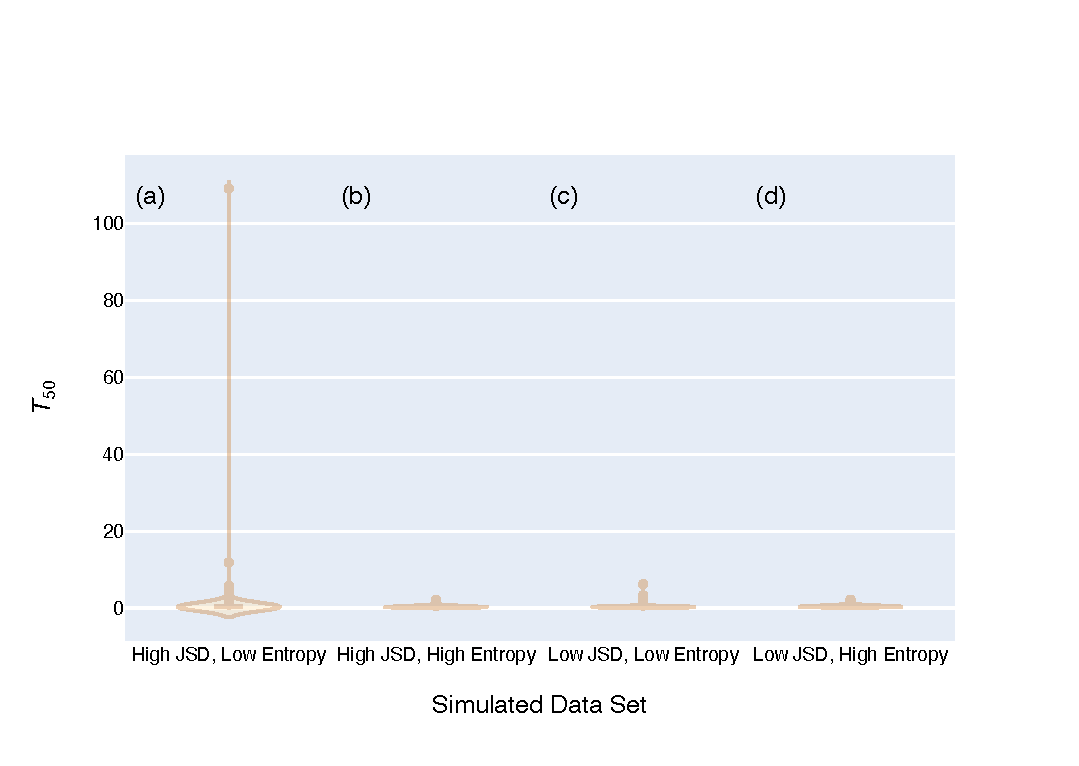
\includegraphics[width=\textwidth]{figures/plots/synthetic/T50/300bp.pdf}
\caption{\textbf{Low Entropy, High JSD data has sampling error for T50 estimates}}
\label{fig:t50_long}
\end{figure}

\begin{figure}[!ht]
\centering
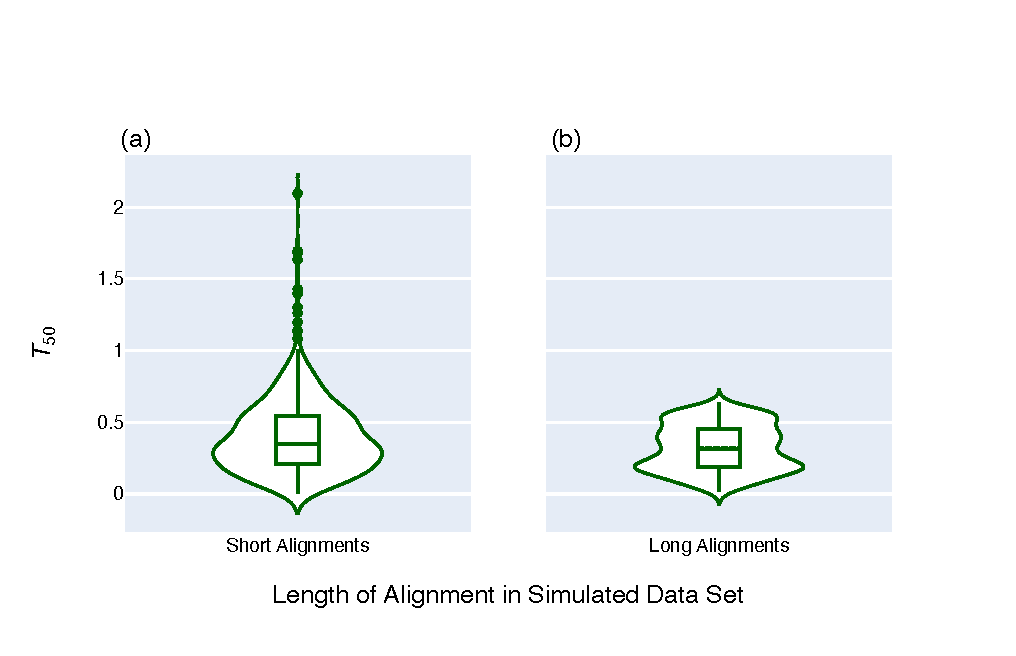
\includegraphics[width=\textwidth]{figures/plots/synthetic/T50/197113_332182_17210-seq_len.pdf}
\caption{\textbf{Long Alignments have less sampling error}}
\label{fig:T50-short_long}
\end{figure}

\subsection{Convergence}

\begin{figure}[!ht]
\centering
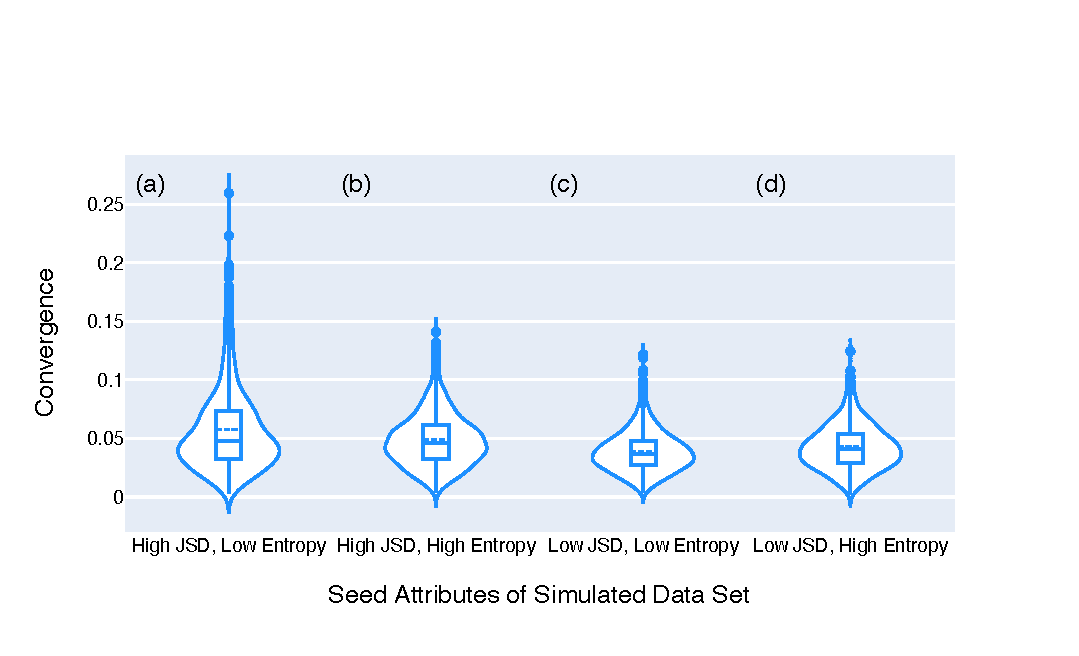
\includegraphics[width=\textwidth]{figures/plots/synthetic/convergence/300bp.pdf}
\caption{\textbf{Short Low Entropy, High JSD alignments exhibit more variance for convergence estimates }}
\label{fig:convergence-short}
\end{figure}

\subsection{Equivalence of Process}

\section{Is the Human Genome at Equilibrium?}

\section{Is the \textit{D. melanogaster} genome further from equilibrium than \textit{D. simulans}?}

\section{Is the half of \textit{Fxy} located in the Psuedo-Autosomal Region (PAR) further from equilibrium than the non-PAR half in \textit{M. musculus}?}